%%%%%%%%%%%%%%%%%%%%%%%%%%%%%%%%%%%%%%%%%%%%%%%%%%%%%%%%%%%%%%%%
\section{Algebraic Loop Resolution}
\label{sec:impl_algebraic_loops}

The algebraic-loop implementation realizes \ref{req:SR-11-03} under \ref{req:UR-11}.
It uses the SCC-local loop blocks detected by the structural analysis of Section~\ref{sec:impl_structural}.
The theoretical basis is introduced in Section~\ref{sec:235_cosim_algebraic_loops}.
When a master algorithm reaches a loop generation, \syssimx{} computes mutually consistent interface values before any component in the loop block advances its state.
The local solver \pyfn{solve\_algebraic\_scc\_ijcsa()} performs this correction for one strongly connected component.
The global \texttt{IJCSAAlgorithm} solves the complete zero-delay interface and is described in Section~\ref{sec:impl_algorithms}.

%%%%%%%%%%%%%%%%%%%%%%%%%%%%%%%%%%%%%%%%%%%%
\subsection{Scope and Local Interface Data}
\label{sec:impl_algebraic_loops_scope}

The local solver operates on a single \ac{SCC} $\mathcal{L}$ and reuses the structural metadata stored on the \texttt{System} instance.
From the zero-delay connections incident to $\mathcal{L}$ it derives four artifacts that together define the local interface problem.
The first artifact is the vector of interface unknowns
\begin{equation}
  U_{\mathcal{L}} = \bigl(u_1,\ldots,u_n\bigr)^\top,
\end{equation}
which collects every destination input port of a zero-delay connection whose source and destination components both belong to $\mathcal{L}$.
The second artifact is a map \pyfn{driver\_for\_input} that resolves each entry of $U_{\mathcal{L}}$ to the source output port that drives it inside $\mathcal{L}$.
The third artifact is the set of internal connections, which are the zero-delay edges with both endpoints in $\mathcal{L}$ and which couple the unknowns through component outputs.
The fourth artifact is the set of external incoming connections, which are zero-delay edges that enter $\mathcal{L}$ from components in earlier generations.
Their driver outputs are read once at the current communication point and kept fixed during the local solve, so they contribute known right-hand-side values rather than additional unknowns.

%%%%%%%%%%%%%%%%%%%%%%%%%%%%%%%%%%%%%%%%%%%%
\subsection{Residual Evaluation}
\label{sec:impl_algebraic_loops_residual}

For a trial vector $U_{\mathcal{L}}$, the solver assembles temporary inputs for every component in $\mathcal{L}$.
These inputs contain the trial values and the fixed external values.
The solver then calls \pyfn{evaluate\_outputs(inputs)} on each component.

Routing the returned outputs through \pyfn{driver\_for\_input} yields the induced interface vector $\widehat{U}_{\mathcal{L}}(U_{\mathcal{L}})$.
The residual is
\begin{equation}
  \mathcal{R}_{\mathcal{L}}(U_{\mathcal{L}}) = U_{\mathcal{L}} - \widehat{U}_{\mathcal{L}}(U_{\mathcal{L}}),
\end{equation}
which matches the fixed-point form of Section~\ref{sec:235_cosim_algebraic_loops} restricted to $\mathcal{L}$.
A consistent loop state is reached when $\|\mathcal{R}_{\mathcal{L}}\|_2$ falls below the solver tolerance.
Because \pyfn{evaluate\_outputs()} does not advance component state, the residual can be sampled at several trial vectors within one macro step.

%%%%%%%%%%%%%%%%%%%%%%%%%%%%%%%%%%%%%%%%%%%%
\subsection{Newton Iteration and Commit}
\label{sec:impl_algebraic_loops_newton}

The iteration starts from the values currently stored in the destination input ports of $\mathcal{L}$.
These values are the most recent consistent inputs from the previous macro step.
Each iteration approximates the interface Jacobian column-wise by forward finite differences,
\begin{equation}
  J^{(m)}_{:,j} \approx
  \frac{
    \mathcal{R}_{\mathcal{L}}\!\bigl(U_{\mathcal{L}}^{(m)} + \varepsilon e_j\bigr)
    - \mathcal{R}_{\mathcal{L}}\!\bigl(U_{\mathcal{L}}^{(m)}\bigr)
  }{\varepsilon},
  \qquad \varepsilon = 10^{-6},
\end{equation}
and applies the standard Newton update $U_{\mathcal{L}}^{(m+1)} = U_{\mathcal{L}}^{(m)} - \bigl(J^{(m)}\bigr)^{-1}\mathcal{R}_{\mathcal{L}}(U_{\mathcal{L}}^{(m)})$.

The loop terminates when $\|\mathcal{R}_{\mathcal{L}}\|_2<\texttt{tol}$.
If the Jacobian is singular or the residual fails to converge within \texttt{max\_iter} iterations, the solver aborts the current macro step with a runtime error rather than committing inconsistent inputs.
The Jacobian becomes singular when the loop-gain eigenvalue approaches one, for example for an identity feedback $y=u$ or a unit-gain cycle.
Finite-difference noise at discontinuities can produce the same condition numerically.

After convergence the solver writes the solved entries of $U_{\mathcal{L}}$ back to the corresponding destination input ports through \pyfn{inputs[dst].set(value, t)}, so the loop inputs are mutually consistent at the current communication point while the component states are still unchanged.
The active master algorithm then performs the subsequent macro step on the basis of these committed values.

%%%%%%%%%%%%%%%%%%%%%%%%%%%%%%%%%%%%%%%%%%%%
\subsection{Verification Scenario}
\label{sec:impl_algebraic_loops_verification}

The verification scenario of Figure~\ref{fig:algebraic_loop_verification} consists of a constant source, two subtractors, and one integrator.
The labels on the ports define the notation used below.

\begin{figure}[H]
  \centering
  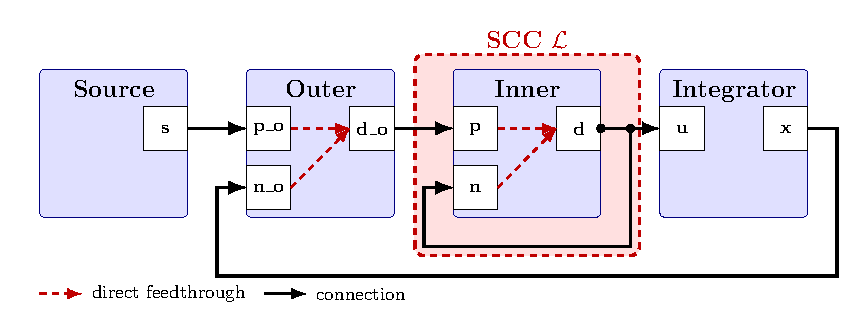
\includegraphics[width=0.9\linewidth]{figures/5_implementation/algebraic_loop/algebraic_loop_verification.pdf}
  \caption{Verification scenario for algebraic loops. The dashed red rectangle marks the SCC node set $\mathcal{L}=\{\texttt{Inner}\}$. Wire routing is purely visual and does not indicate SCC membership.}
  \label{fig:algebraic_loop_verification}
\end{figure}

The \texttt{Source} emits $s=1$.
The two subtractors \texttt{Inner} and \texttt{Outer} are direct-feedthrough components with output equation $d_o=p_o-n_o$ and $d=p-n$ respectively.
The \texttt{Integrator} advances $\dot{x}=u$ with $x(0)=0$ and has no feedthrough.
Five connections close the topology.
The source drives the positive input of \texttt{Outer}.
The output of \texttt{Outer} drives the positive input of \texttt{Inner}.
The output of \texttt{Inner} drives the integrator input and is also fed back to its own negative input.
The integrator output drives the negative input of \texttt{Outer}.
This last connection is delayed because the integrator has no direct feedthrough from $u$ to $x$.

The self-connection $d\to n$ is the only zero-delay cycle, so the structural analysis stores a single SCC $\mathcal{L}=\{\texttt{Inner}\}$.
For the local solve, $n$ is the only interface unknown and the edge $d_o\to p$ appears as the one external incoming connection held fixed at the current communication point.
At $t=0$ the integrator output is zero, so the external value reduces to $p=s-x=1$.
The local problem collapses to the scalar fixed-point equation $n=p-n$ with analytical solution $n=d=\tfrac{1}{2}p=0.5$.

\begin{listing}[ht]
  \begin{lstlisting}[
    basicstyle=\ttfamily\footnotesize,
    frame=single,
    backgroundcolor=\color{black!3},
    breaklines=true,
    columns=fullflexible,
    xleftmargin=0pt
]
Solving algebraic SCC ['Inner']:
  Interface inputs:                [('Inner', 'neg')]
  Internal zero-delay connections: [('Inner', 'diff', 'Inner', 'neg')]
  External zero-delay inputs:      [('Outer', 'diff', 'Inner', 'pos')]
  Initial guess for Inner.neg = -0.001
Starting IJCSA iterations:
  Iteration 0: u = [-0.001]
    Residual for Inner.neg: -1.0019999999999998
    Jacobian J = [[2.]]
    Correction du = [0.501]
  Iteration 1: u = [0.5]
    Residual for Inner.neg: 8.243e-11
  Converged in 1 iterations.
Committed solved input Inner.neg = 0.5000000000412155
\end{lstlisting}
  \caption{IJCSA solver trace for the algebraic-loop verification scenario.
    The local solver identifies the scalar interface problem and converges to the analytical solution in one Newton step.}
  \label{lst:ijcsa_verification_log}
\end{listing}

Listing~\ref{lst:ijcsa_verification_log} confirms the expected local interface problem.
The solver identifies one interface unknown, one internal self-connection, and one external incoming zero-delay input.
Starting from the initial guess, it converges to $n=0.5$ in one Newton step and commits the value before the macro step.
This agrees with the analytical solution and verifies the SCC-local loop solve.